%Capítulo 2

    En este capítulo, veremos la situación en la que se encuentra el estado del arte en la educación Pública del estado de Jalisco, se nombrarán los objetivos detectados del acuerdo número 11/03/19 del Diario Oficial de la Federación \cite{sep} que pone las bases sobre el cual se evalua el aprendizaje de los alumnos en el ambiente escolar. \\ Además se hará una actualización de la comparativa de la oferta que se tiene de aplicaciones que se dedican a mejorar el ámbito educativo, las cuáles pueden tener un objetivo similar al nuestro de ayudar al alumno a mejorar su desempeño academico de los alumnos. \\ Como se menciona las aplicaciones ofrecen servicios parecidos pero estos serán analizados utilizando las caracteristicas principales que se cree son las mejores para categorizar el nivel de apoyo que dan dichas aplicaciones realmente a los alumnos y los resultados que estas pudieran tener en escuelas.

    \section{Situación actual}
    
        Basándonos en el acuerdo número 11/03/19 del Diario Oficial de la Federación \cite{sep}, en el cual se establecen las normas generales para la evaluación de los aprendizajes esperados, acreditación, regularización, promoción y certificación de los educandos de la educación básica \cite{sep}, podemos extraer los siguientes puntos más relevantes:
    
        \begin{itemize}
            \item Los resultados de la evaluación del aprendizaje habrán de analizarse con estudiantes, madres y padres de familia o tutores, así como por las autoridades escolares y educativas, como base para acordar acciones que cada parte debe realizar para mejorar el desempeño de niñas, niños o adolescentes, según corresponda en cada caso
            
            \item En la aplicación de las presentes normas deberá garantizarse la participación activa de todos los involucrados en el proceso educativo: autoridades educativas y escolares, docentes, madres, padres de familia o tutores y educandos
            
            \item La comunicación a las madres y padres de familia o tutores de los resultados de las evaluaciones parciales, y la entrega de la Boleta de Evaluación al final del ciclo escolar, no limita su derecho a informarse sobre el desempeño y desarrollo de sus hijos o pupilos en cualquier momento. Tampoco limita a los docentes y directivos para convocar a los padres de familia o tutores a la escuela cuando lo consideren necesario
            
        \end{itemize}
        

    \section{Aplicaciones no comerciales}
    
        Durante la investigación del estado del arte se encontraron múltiples soluciones que pretenden servir como apoyo del maestro, los alumnos y los padres de familia. También cabe mencionar se evaluará lo realizado previamente con la aplicación móvil Eduintegral \cite{eduintegral} y se analizarán los puntos que se lograrón cubrir. \\ En esta sección se analizaran todas las caracteristicas de dichas aplicaciones y se compararán de manera directa para observar de manera rápida el estado del arte en el que se encuentran.


        \subsection{Consulta escolar Jalisco}
        
            La secretaría pública del estado de Jalisco ofrece una aplicación móvil llamada ``Consulta escolar Jalisco'', la cuál puede ser encontrada con el siguiente logo dentro de la play store de Google (ver Figura 2.1):
            
            \begin{figure}[H]
                \centering
                
\includegraphics[scale=0.3]{imagenes/consulta_escolar_jalisco.png}
                \caption{Consulta escolar Jalisco}
                \label{fig:consultaescolarjalisco}
            \end{figure}
            
            Esta aplicación permite a los padres de familia y tutores, consultar los avances de los alumnos de escuelas públicas del estado de Jalisco. \\ También se podrá realizar la inscripción en línea anualmente al ciclo escolar correspondiente, así como recibir automáticamente las calificaciones bimestrales del alumno en el correo electrónico registrado y descargar su certificado digital al termino de su nivel educativo \cite{consulta}. \\ Dada la funcionalidad que ofrece la apliación se considera que es la que puede competir de manera más directa con lo que se pretende hacer en este proyecto. \\ Esta aplicación se encuentra disponible de manera gratuita en dispositivos Android, la aplicación cuenta con más de 100,000 descargas desde la Play Store. \\ Una de sus funciones principales es la de servir como un portal de acceso para obtener el historial academico de los alumnos, más aparte se puede considerar que tiene buena seguridad visto desde del punto de vista que la aplicación es manejada por el estado de Jalisco, también por lo mismo se considera que no permite el acceso a ser administrada por otras partes. \\ En la siguiente imagen se puede apreciar dos pantallas de acceso de la aplicación (ver figura 2.2).
            
            \begin{figure}[H]
                \centering
                
\includegraphics[scale=0.8]{imagenes/consulta_escolar_jalisco_2.png}
                \caption{Pantalla de preinscripciones, descarga de certificado y consulta de calificaciones}
                \label{fig:consultaescolarjalisco2}
            \end{figure}

        \subsection{Eduintegral}

            La aplicación Eduintegral \cite{eduintegral} es capaz de conectar a los padres de familia con el maestro, más sin embargo al encontrarse todavía en desarrollo tiene de momento deficiencias de diseño y estructura visual. La aplicación móvil fue probada en un ambiente totalmente virtualizado junto con un servidor con una carga simulada esto dado que no se contó con un servidor real con el cuál hacer las pruebas. \\ Durante las pruebas se detectaron un sin número de errores los cuales fueron solucionados en su mayoría dando pie a que la aplicación pudiera capturar y leer registros de la base de datos. Lamentablemente el tiempo de desarrollo no fue suficiente para terminar todas las funcionalidades planeadas lo cual se dejo como trabajo futuro. \\ En cuanto a la propuesta que se realizo en su momento se búsco enfocarse en una herramienta que fuera lo más fácilmente de usar posible, pensando en aspectos como el económico, el de una infraestructura básica y que la aplicación fuera intuitiva para los padres de familia y maestros. Esta aplicación móvil fue hecha y pensada con el punto de vista de maestros profesionales en la educación que trabajan directamente en campo y de los cuales se obtuvieron puntos de vista, opiniones y propuestas que ayudaron bastante en el desarrollo de este proyecto \cite{eduintegral}. La pantalla de inicio de Eduintegral pide usuario y contraseña, además de identificar desde un principio si se trata de un padre de familia o un maestro (ver figura 2.3). 
            
            \begin{figure}[H]
                \centering
                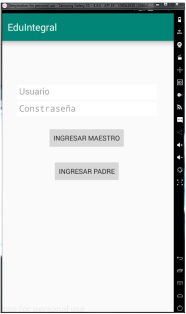
\includegraphics[scale=0.9]{Propuesta_Plantilla_Tesis_LaTeX_UAG/imagenes/eduintegral.png}
                \caption{Eduintegral}
                \label{fig:eduintegral}
            \end{figure}


    \section{Aplicaciones comerciales}
        
        Dentro del ámbito escolar también se encuentran aplicaciones comerciales las cuales al detectar la problematica que existe acerca del desempeño estudiantil y de la desconexión del núcleo familiar con respecto a la escuela, intentan tambien proveer una solución, trayendo consigo multiples funcionalidades y un sistema de mayor competencia, lo cual se cree es algo bueno para la causa de los alumnos. A continuación se presentan algunas de las aplicaciones móviles más relevantes del mercado.
    
        
        \subsection{Schoolway}
        
            Disponible para teléfonos inteligentes con sistema operativo Android y iOS, la aplicación se puede descargar de manera gratuita contactando directamente al desarrollador, dado que ya no se encuentra disponible en la Play Store de momento, la escuela que este interesada en la aplicación tiene que pagar una suscripción para poder usarla \cite{schoolway}. \\ La aplicación es capaz de conectar alumnos, escuela y a los padres de familia dentro de la misma comunidad estudiantil. Da avisos generales utilizando notificaciones push ilimitadas, que inclusive pueden ser programadas con antelación, se pueden crear grupos dentro de la aplicación. \\ La administración y el acceso a la base de datos se considera que es cerrada dado que el control total de la aplicación es solo por parte del desarrollador. La siguiente imagen muestra el logo de la aplicación firmado por su desarrollador (ver figura 2.4).

            \begin{figure}[H]
                \centering
                
\includegraphics[scale=3.0]{Propuesta_Plantilla_Tesis_LaTeX_UAG/imagenes/schoolway.png}
                \caption{Jostens schoolway}
                \label{fig:schoolway}
            \end{figure}


        \subsection{Edmodo for parents}
        
            Aplicación móvil disponible para teléfonos inteligentes con sistema operativo Android y iOS, la cual se puede descargar de manera gratuita desde las tiendas digitales oficiales. La antigua imagen de edmodo se puede apreciar en la siguiente imagen (ver figura 2.5).
        
            \begin{figure}[H]
                \centering
                
\includegraphics[scale=0.2]{Propuesta_Plantilla_Tesis_LaTeX_UAG/imagenes/edmodo.jpeg}
                \caption{Edmodo for parents}
                \label{fig:edmodo}
            \end{figure}
        
            La aplicación actual cuenta con más de 10 millones de descargas en la Play Store, la aplicación pone a disposición del maestro el poder avisar a los padres de familia acerca de tareas, presentaciones y anuncios de maestros. Los padres de familia son más aparte capaces de consultar la información sobre calificaciones y actividades del alumno. La administración y el acceso a la base de datos se considera cerrado dado que esa parte de la aplicación solo puede ser manejada por el desarrollador. La aplicación opera sobre un modelo freemium lo cual significa que parte del uso es gratuito pero para obtener algunas funcionalidades se tiene que pagar una cuota. Edmodo rediseño su imagen en general, creando a su vez un nuevo logo (ver figura 2.6) \cite{edmodo}.
        
            \begin{figure}[H]
                \centering
                
\includegraphics[scale=0.2]{Propuesta_Plantilla_Tesis_LaTeX_UAG/imagenes/edmodo.png}
                \caption{Edmodo for parents nuevo logo}
                \label{fig:edmodo}
            \end{figure}


        \subsection{ClassDojo}
        
            ClassDojo se encuentra disponible para dispositivos móviles con sistema operativo Android y iOS, la aplicación se puede descargar en la tienda digital de dichos sistemas operativos. La aplicación aclama que el uso es gratuito por siempre para maestros que la quieran usar, más sin embargo para poder acceder al contenido premium se requiere pagar por el mismo, más aparte cuenta con un servicio de pago mensual con algunas opciones extra. \\ ClassDojo cuenta con mas de 10 millones de descargas en la Play Store, siendo esta una aplicación muy popular (ver figura 2.7) \cite{classdojo}. 
            
            \begin{figure}[H]
                \centering
                
\includegraphics[scale=0.2]{Propuesta_Plantilla_Tesis_LaTeX_UAG/imagenes/classdojo.jpg}
                \caption{ClassDojo}
                \label{fig:classdojo}
            \end{figure}
            
            La aplicación cuenta con una especie de salón de clases virtual utilizando la nube, al salón virtual pueden ser invitados los padres de familia de los alumnos que ya se encuentren dentro. A los integrantes del salón la aplicación les permite compartir fotos, videos y anuncios al mismo salón. La administración y acceso a la base de datos es permitida sólo por el desarrollador \cite{classdojo}. 
    
    
        \subsection{Remind-School Communication}
        
            La aplicación Remind-School Communication se encuentra disponilbre para teléfonos inteligentes con sistema operativo Android y iOS, esta se puede descargar de manera gratuita desde las tiendas digitales oficiales. \\ Ofrece a los maestros una forma sencilla y segura para enviar SMS a estudiantes y padres de familia, la aplicación aclama que es segura porque mantiene de forma segura los números de telefono. También permite a maestros, monitores o administradores el envio de recordatorios, tareas, actividades, evaluaciones y mensajes motivadores. La administración de la aplicación y el acceso a la base de datos es por parte del desarrollador por lo cual el acceso es cerrado. \\ La descarga y el uso básico de la aplicación es gratuito, también cuenta con un plan premium el cuál es de paga.La aplicación cuenta con mas de 10 millones de descargas desde la Play Store (ver figura 2.8) \cite{remind}.
            
            \begin{figure}[H]
                \centering
                
\includegraphics[scale=0.4]{Propuesta_Plantilla_Tesis_LaTeX_UAG/imagenes/remind.png}
                \caption{Remind-School Communication}
                \label{fig:remind}
            \end{figure}


    \section{Discusión de otras aplicaciones}
    
    Revisado las aplicaciones analizadas se pueden inicialmente dividir en aplicaciones comerciales y apliciones no comerciales, lo cual indica ya en si una diferencia en cuanto a que unas aplicaciones limitaran la funcionalidad que se otorga ha no ser de que se realice un pago mensual mientras que las aplicaciones no comerciales otorgan todas las funcionalidades de manera completa y sin costo, aunque tambien cabe mencionar que las apliciones comerciales mostraron generalmente tener muchas funciones extras. \\ Se puede deducir que todas las apliciones si llegan a proporcionar en cierto grado una comunicación entre padres de familia y maestros, haciendo uso de las notificiones push proporcionadas por el sistema y de grupos generados en base a los grupos escolares de las escuelas. La mayoría de las aplicaciones se encuentran disponibles al momento de realizar este proyecto, tambien cabe mencionar que se observo que el uso de las aplicaciones comerciales sobre pasa por mucho el uso de las aplicaciones no comerciales, dando cifras por millones de usuarios de diferencia, aunque en el caso de Eduintegral, esta todavía no se encuentra dispobile al público. \\ Aunque para el caso de estudio de este proyecto cabe mencionar que la cantidad de usuarios activos o de paga no es relevante. El punto negativo de todas las aplicaciones comerciales es el cobro de una cuota mensual para el uso de las funcionalidades premium o para acceder a contenido especial. También se observo que con las aplicaciones comerciales no se tiene autorizado por parte de los desarrolladores el acceso a las bases de datos de las aplicaciones, también la administración de las mismas aplicaciones se vio mermada por esta situación dado que esta cerrada para terceros. \\ La seguridad y privacidad que puede tener la información de todos los usuarios por parte de las aplicaciones comerciales es una incognita dado que los desarrolladores de las mismas mantienen en privado dicha información y no se dan más detalles.
    Finalmente, se puede decir que el enfoque de las aplicaciones comerciales va más dirigido a las actividades y tareas llevadas en el salón de clases que en mejorar la comunicación entre padres de familia y maestros. Dadas todas estas caracteristicas y detalles observados durante la investigación se generó la siguiente tabla comparativa, mostrando de manera clara y concisa todos los puntos evaluados según el objetivo de este trabajo (ver tabla 2.1) \cite{eduintegral}.
        
        \begin{table}[H]
            \centering
            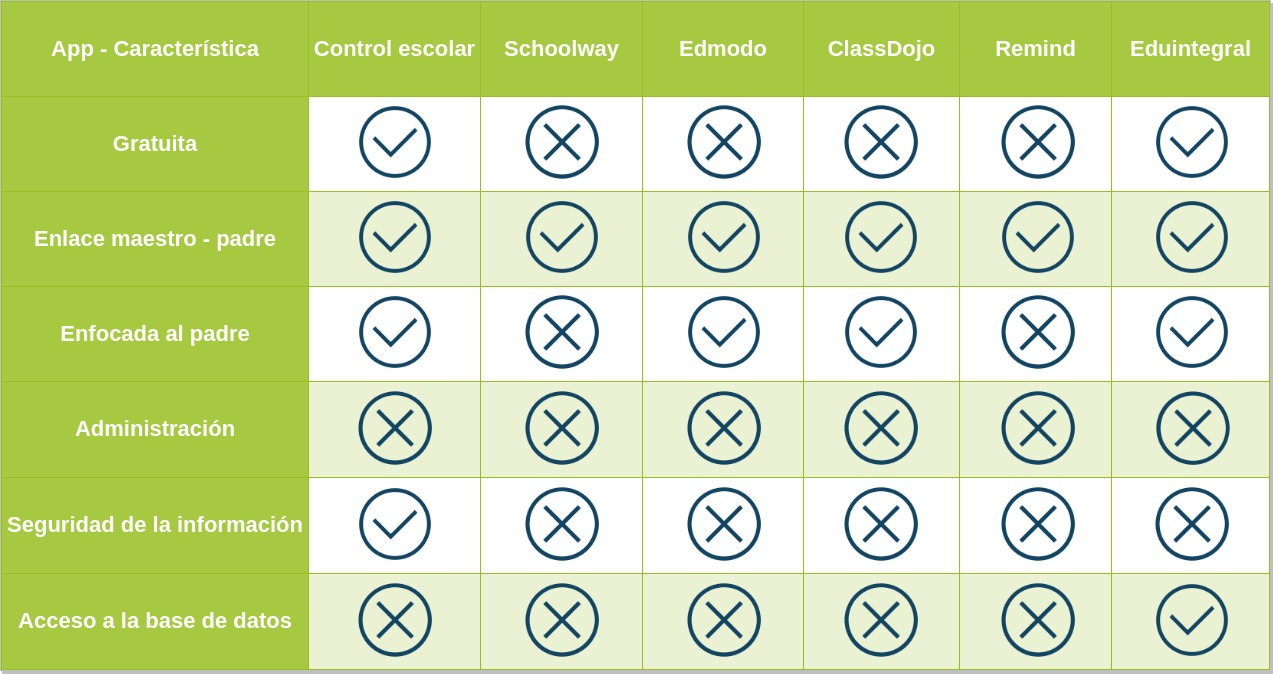
\includegraphics[scale=0.3]{Propuesta_Plantilla_Tesis_LaTeX_UAG/imagenes/tabla_comparativa_de_aplicaciones.jpg}
            \caption{Tabla comparativa de aplicaciones}
            \label{tab:comparativa}
        \end{table}
        
        \begin{itemize}
            \item \textbf{Gratuita:} Se refiere a si la aplicación se puede descargar y usar de manera gratuita por todos los involucrados
            
            \item \textbf{Enlace maestro-padre:} Indica si la aplicación logra la comunicación directa, total o parcialmente, entre padres de familia y el maestro
            
            \item \textbf{Enfocada al padre:} Nos dice si la aplicación está enfocada, diseñada y dirigida para uso especı́fico del padre de familia, tomando en cuenta sus requerimientos más importantes sobre otras funciones que no sean tan necesarias \cite{eduintegral}
            
            \item \textbf{Administración:} Describe si la aplicación permite ser administrada y adaptada a las necesidades particulares de las escuelas
            
            \item \textbf{Seguridad de la información:} Analiza si la información que se propociona a la aplicación y por ende al desarrollador está resguardada de manera segura, si se menciona en dónde será almacenada, cómo se resguarda y por último si el uso que se le dará a dicha información es mencionado
            
            \item \textbf{Acceso a la BD:} Muestra si al usar la aplicación podemos tener acceso a los datos recabados en la base de datos para efectos de análisis y/o estadı́sticos o si en todo caso podemos resguardar nuestros propios datos en una base de datos local.
            
        \end{itemize}
